\documentclass[10pt,a4paper]{article}
\usepackage[margin=20mm]{geometry}
\usepackage[T1]{fontenc}
\usepackage{lmodern,graphicx,booktabs,array,amsmath,hyperref,float,multirow}
\hypersetup{colorlinks=true,urlcolor=blue,linkcolor=blue}
\setlength{\parindent}{0pt}\setlength{\parskip}{5pt}
\newcommand{\uF}{\ensuremath{\mu}F}
% generated by scripts/dclink_report.py
\newcommand{\BLocalCap}{0.88}
\newcommand{\BRowOne}{1.31}
\newcommand{\BRowTwo}{1.33}
\newcommand{\BRowThree}{1.39}
\newcommand{\BExt}{18.4}
\newcommand{\BWLocalCap}{0.87}
\newcommand{\BWRowThree}{1.54}
\newcommand{\BWExt}{43.1}
\newcommand{\PcapRatedBus}{0.186}
\newcommand{\Ipk}{141}
\newcommand{\IlegWorst}{50.0}
\newcommand{\IlegWorstM}{0.05}
\newcommand{\IlegWorstPf}{0.0}
\newcommand{\IlegRated}{28.8}
\newcommand{\ItotWorst}{65.0}
\newcommand{\ItotWorstM}{0.60}
\newcommand{\ItotWorstPf}{1.0}
\newcommand{\ItotRated}{50.3}
\newcommand{\KlegV}{707}
\newcommand{\KtotV}{700}
\newcommand{\KlegSimple}{707}
\newcommand{\CLegFifty}{471}
\newcommand{\CTotFifty}{467}
\newcommand{\CBlockFifty}{156}
\newcommand{\CBlockFiftyThree}{78}
\newcommand{\LfFifty}{150}
\newcommand{\LfFive}{15.0}
\newcommand{\ShLocal}{10.54}
\newcommand{\ShLocalCap}{0.88}
\newcommand{\ShRowOne}{1.28}
\newcommand{\ShRowTwo}{1.29}
\newcommand{\ShRowThree}{1.36}
\newcommand{\WLocalCap}{0.89}
\newcommand{\WRowOne}{2.03}
\newcommand{\WRowTwo}{2.04}
\newcommand{\WRowThree}{2.08}
\newcommand{\PcapRated}{0.179}
\newcommand{\PcapWorst}{0.360}

% generated by scripts/dclink_report.py
\newcommand{\CreqRows}{%
20\,kHz & 2357 & 778 (258) & 1178 & 389 (128) & 589 & 194 (64) \\
50\,kHz & 943 & 311 (102) & 471 & 156 (51) & 236 & 78 (25) \\
100\,kHz & 471 & 156 (51) & 236 & 78 (25) & 118 & 39 (12) \\
200\,kHz & 236 & 78 (25) & 118 & 39 (12) & 59 & 19 (5) \\
}


\title{DC-link capacitor sizing\\[2pt]\large 75\,V, 100\,A$_\mathrm{rms}$ GaN phase leg (2\,$\times$\,EPC2361 per switch)}
\author{PCB-Design project, KTH}
\date{6 October 2026 --- design study}

\begin{document}
\maketitle

\begin{abstract}
The DC-link capacitor of the symmetric EPC2361 phase-leg building block is sized from the switching-frequency current it must supply.
RMS ripple currents are derived analytically and checked with a time-domain PWM model for a single leg and for three legs sharing one bus, over modulation index and power factor.
The required effective capacitance is given versus allowed voltage ripple for 20--200\,kHz.
Finally, the ripple current is split between the individual capacitors using the Q3D-extracted copper of the building block.
Main results: worst-case ripple current \IlegWorst\,A$_\mathrm{rms}$ for a leg on its own and \ItotWorst\,A$_\mathrm{rms}$ for a three-phase bus; at 50\,kHz a $\pm$2\,\% (3\,V\,pp) ripple needs \CBlockFiftyThree\,\uF{} effective per leg on a shared bus, which the selected 24\,$\times$\,10\,\uF{} + 12\,$\times$\,1\,\uF{} bank provides; each capacitor carries at most about 2\,A$_\mathrm{rms}$.
\end{abstract}

\section{Assumptions and definitions}
\begin{itemize}\itemsep0pt
\item $V_\mathrm{dc}=75$\,V, sinusoidal phase current $I=100$\,A$_\mathrm{rms}$ ($\hat I=\Ipk$\,A), ideal switches, no dead time.
\item Modulation: SVPWM (min--max zero sequence), common triangular carrier for all legs; analytical formulas are for SPWM.
\item The DC source or bulk capacitor supplies the switching-period average of the input current; the DC-link capacitor supplies the rest (``HF'' current). For a three-phase inverter the average input power is constant, so no low-frequency ripple appears.
\item ``Single leg'': a leg's own capacitors supply its own HF current (blocks far apart, or a stand-alone leg). ``Three legs'': three legs share one bank, so their HF currents partly cancel.
\item Modulation index $M = \hat V_\mathrm{phase}/(V_\mathrm{dc}/2)$, $0\dots1.15$; power factor $\cos\varphi = 0\dots1$.
\end{itemize}
Script: \texttt{scripts/dclink\_report.py} (all numbers and figures in this report).

\section{RMS ripple current}
With switching function $s_k\in\{0,1\}$ and phase current $i_k$, the input current of leg $k$ is $i_{\mathrm{in},k}=s_k i_k$, with switching-period average $d_k i_k$. Its HF part has the period-mean square $d_k(1-d_k)\,i_k^2$.

\textbf{Single leg (SPWM).} With $d=\tfrac12(1+M\sin\theta)$ and $i=\hat I\sin(\theta-\varphi)$, averaging over the fundamental:
\begin{equation}
I_{C,\mathrm{leg}} = \frac{\hat I}{2}\sqrt{\frac12 - M^2\left(\frac14+\frac{\cos 2\varphi}{8}\right)}
\end{equation}
It is largest at low $M$: $\hat I/(2\sqrt2)=$\,\IlegWorst\,A for 100\,A$_\mathrm{rms}$. At the rated point ($M=1$, $\cos\varphi=1$) it is \IlegRated\,A.

\textbf{Three legs on one bus (Kolar \& Round).}
\begin{equation}
I_{C,3\phi} = \hat I\sqrt{M\left[\frac{\sqrt3}{4\pi}+\cos^2\varphi\left(\frac{\sqrt3}{\pi}-\frac{9M}{16}\right)\right]}
\end{equation}
Maximum \ItotWorst\,A at $M\approx$\,\ItotWorstM, $\cos\varphi=$\,\ItotWorstPf; \ItotRated\,A at the rated point. This is the total for all three legs, about one third per leg.

\begin{figure}[H]\centering
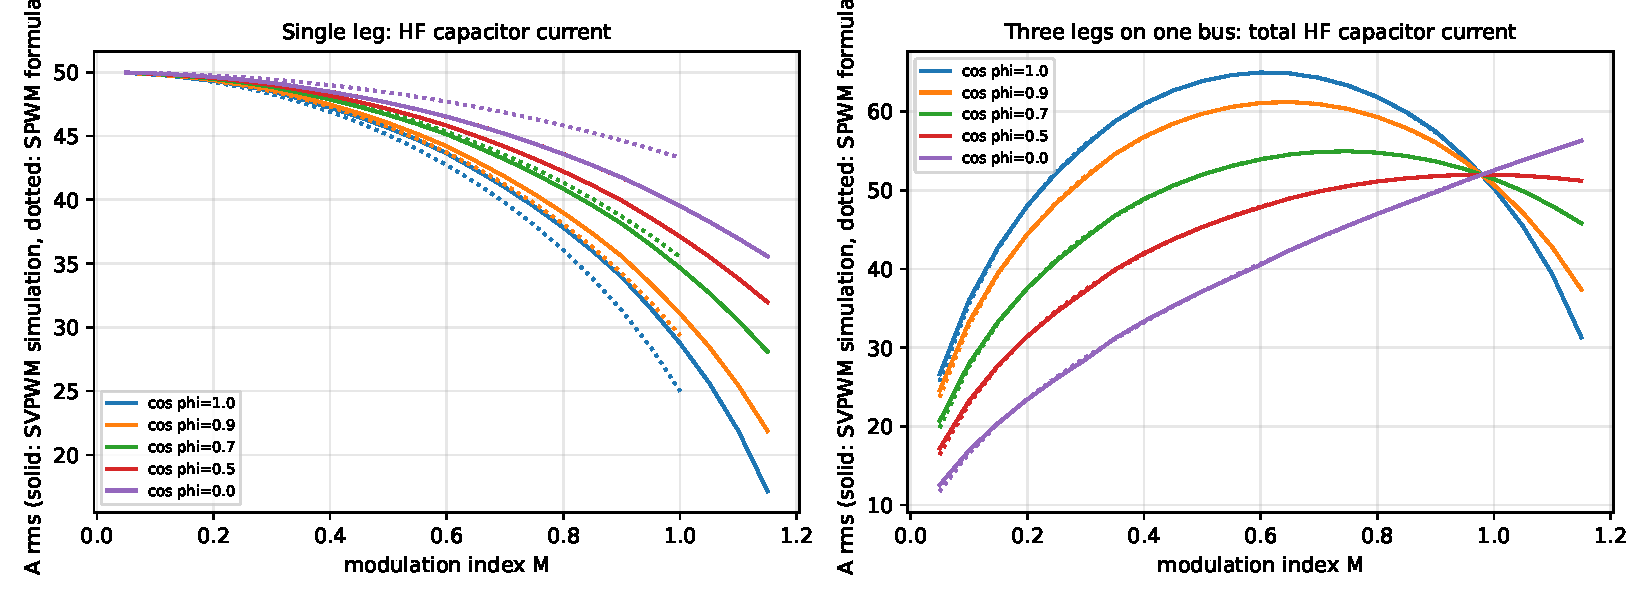
\includegraphics[width=\textwidth]{figures/irms.pdf}
\caption{HF capacitor RMS current versus modulation index. Solid: time-domain SVPWM model; dotted: SPWM formulas above. They agree at low $M$; above $M\approx0.6$ the SVPWM zero sequence changes the duty cycles and the single-leg current is up to about 15\,\% higher than the SPWM formula (\IlegRated\,A vs 25\,A at $M=1$). The three-leg total is almost unaffected.}
\end{figure}

\section{Voltage ripple and required capacitance}
For a capacitor $C$ supplying the HF current, the worst peak-to-peak ripple within a switching period scales as $\Delta V_\mathrm{pp} = K/(f_\mathrm{sw}C)$.
\begin{itemize}\itemsep0pt
\item Single leg: the worst case is $d=0.5$ at the current peak (low $M$), giving the hand formula $\Delta V_\mathrm{pp}=\hat I/(4 f_\mathrm{sw} C)$. At 50\,kHz this is \KlegSimple\,V for 1\,\uF; the PWM model gives \KlegV\,V.
\item Three legs on one bank: the PWM model gives \KtotV\,V for 1\,\uF{} of total capacitance at 50\,kHz (worst over $M$ and $\cos\varphi$). The total bank therefore needs about the same capacitance as one isolated leg, so each of the three blocks needs one third.
\end{itemize}

\begin{figure}[H]\centering
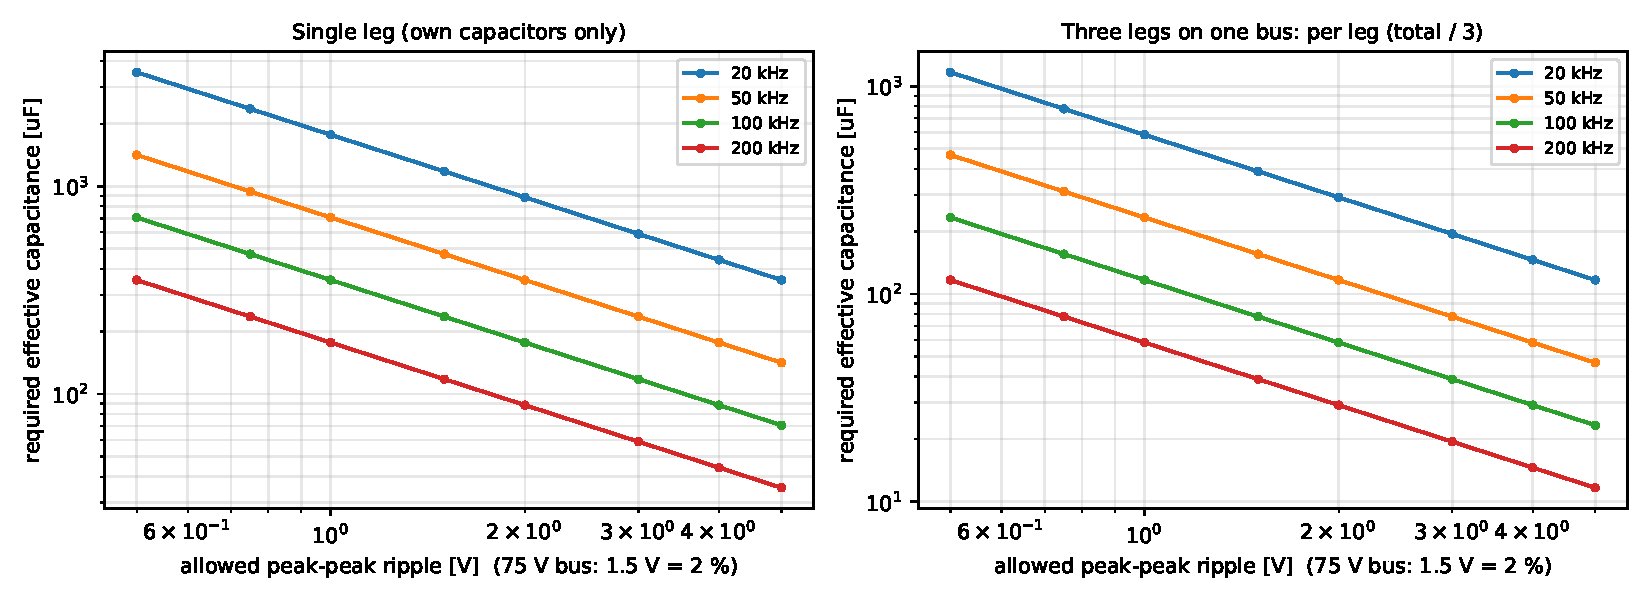
\includegraphics[width=\textwidth]{figures/creq.pdf}
\caption{Required effective capacitance versus allowed peak-peak ripple. Left: single leg with its own capacitors. Right: three legs on one bus, per leg.}
\end{figure}

\begin{table}[H]\centering\small
\begin{tabular}{@{}lcccccc@{}}\toprule
 & \multicolumn{2}{c}{0.75\,V pp ($\pm$0.5\,\%)} & \multicolumn{2}{c}{1.5\,V pp ($\pm$1\,\%)} & \multicolumn{2}{c}{3\,V pp ($\pm$2\,\%)} \\
$f_\mathrm{sw}$ & leg alone & per leg, shared & leg alone & per leg, shared & leg alone & per leg, shared \\\midrule
\CreqRows
\bottomrule\end{tabular}
\caption{Required effective capacitance in \uF. In brackets: number of 10\,\uF{}/100\,V 1210 MLCCs (3\,\uF{} effective at 75\,V) per leg, in addition to the 12 local 1\,\uF{} 0805 parts (5.4\,\uF{} effective).}
\end{table}

\textbf{Selected bank per leg:} 24\,$\times$ Murata GRM32EC72A106KE05L (10\,\uF, 100\,V, X7S, 1210) and 12\,$\times$ TDK C2012X7S2A105K125AB (1\,\uF, 100\,V, X7S, 0805). Assuming 30\,\% and 45\,\% of nominal at 75\,V, this is 77\,\uF{} effective. That meets $\pm$2\,\% at 50\,kHz and $\pm$1\,\% at 100\,kHz on a shared three-phase bus (\CBlockFiftyThree\,\uF{} required). A leg used on its own would need \CLegFifty\,\uF{} for $\pm$1\,\% at 50\,kHz; that is a job for film or polymer capacitors on the DC bus, not for more MLCCs on the block. The DC-bias derating must be confirmed with the manufacturers' data (Murata SimSurfing, TDK SEAT).

\subsection*{Stand-alone single-phase half bridge}
If one leg drives a load returned to the midpoint of a split DC link, each half of the link carries $i/2$ at the fundamental frequency $f_1$. The midpoint ripple is then $\Delta V_\mathrm{pp}\approx \hat I/(2\pi f_1 C_\mathrm{half})$, which needs \LfFifty\,mF per half at 50\,Hz for 3\,V\,pp, or \LfFive\,mF at 500\,Hz. That is electrolytic-bank territory. It is the reason the block is intended for three-phase use, where this ripple cancels.

\section{Capacitor RMS currents}
The leg ripple current is not shared equally: the local 0805 banks sit inside the commutation loop, the 1210 rows are further away, and an external bus may take part of the low-frequency content.
Method: the HF current of leg A from the PWM model is transformed (FFT over one fundamental period; bins holding 99.9\,\% of the energy). Each harmonic is injected between the high-side drains and low-side sources of the Q3D building-block copper model (2\,oz inner layers, inductance and resistance matrices). The copper resistance rises from the DC to the 100\,MHz value as $\sqrt f$. Capacitors: 0805 0.45\,\uF/6\,m$\Omega$/0.48\,nH, 1210 3\,\uF/3\,m$\Omega$/0.5\,nH each. Optional external bus: 20\,nH and 2\,m$\Omega$ to a 1\,mF/20\,m$\Omega$ bulk.

\begin{figure}[H]\centering
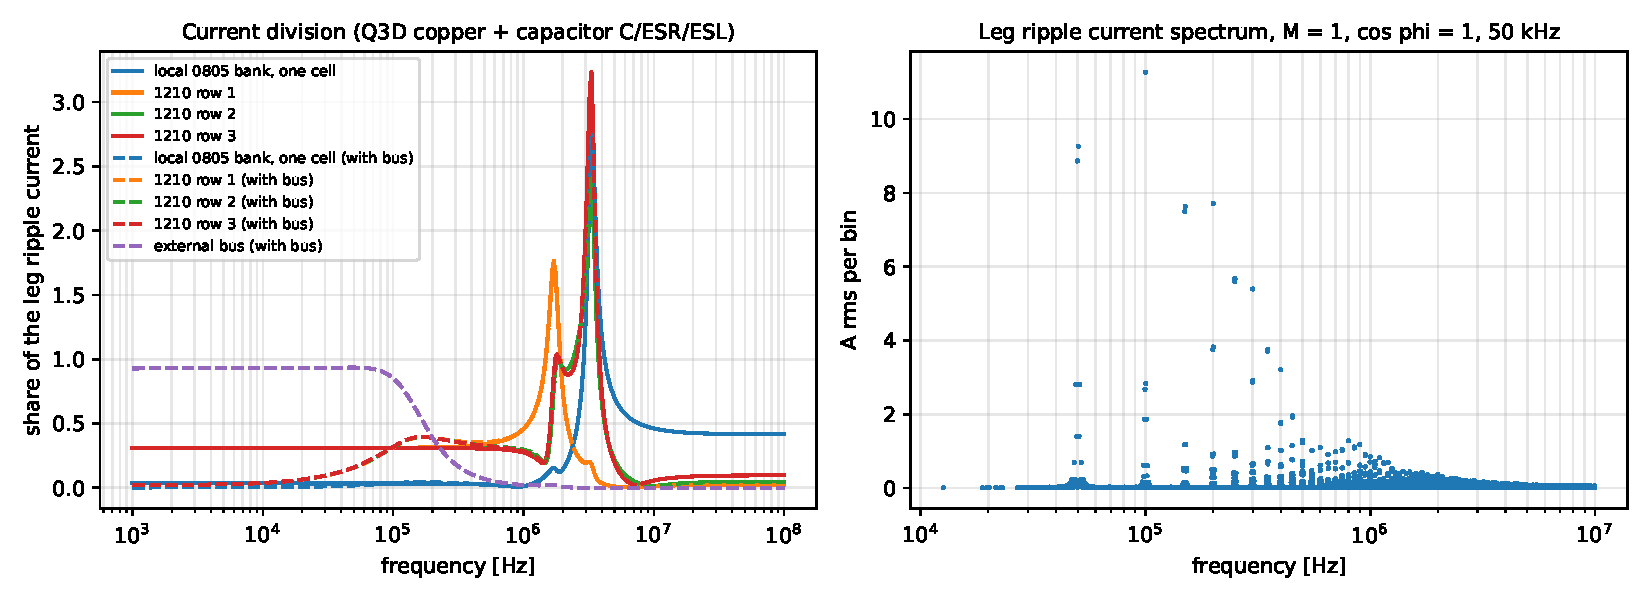
\includegraphics[width=\textwidth]{figures/sharing.pdf}
\caption{Left: fraction of a ripple-current harmonic carried by each capacitor group versus frequency (solid: block alone; dashed: with external bus). Right: ripple-current spectrum of one leg at the rated point.}
\end{figure}

\begin{table}[H]\centering\small
\begin{tabular}{@{}lcccc@{}}\toprule
RMS current per capacitor [A] & \multicolumn{2}{c}{block alone} & \multicolumn{2}{c}{with external bus} \\
 & rated (M=1, $\cos\varphi$=1) & worst (low M) & rated & worst \\\midrule
local 0805, 1\,\uF{} (12 parts) & \ShLocalCap & \WLocalCap & \BLocalCap & \BWLocalCap \\
1210 row 1, 10\,\uF{} (8 parts) & \ShRowOne & \WRowOne & \BRowOne & -- \\
1210 row 2, 10\,\uF{} (8 parts) & \ShRowTwo & \WRowTwo & \BRowTwo & -- \\
1210 row 3, 10\,\uF{} (8 parts) & \ShRowThree & \WRowThree & \BRowThree & \BWRowThree \\
external bus (whole) & -- & -- & \BExt & \BWExt \\
ESR loss, all on-board capacitors [W] & \PcapRated & \PcapWorst & \PcapRatedBus & -- \\
\bottomrule\end{tabular}\end{table}

Observations:
\begin{itemize}\itemsep0pt
\item Each 1210 carries 1.3--2.1\,A$_\mathrm{rms}$ and each 0805 about 0.9\,A$_\mathrm{rms}$. With the assumed ESR this is 5--13\,mW per part, a self-heating of a few kelvin; confirm against the ripple-current rating in the manufacturer data.
\item The external bus mainly takes the switching-frequency fundamental and its first harmonics. At 50\,kHz the 77\,\uF{} bank is about 40\,m$\Omega$, comparable to a 1\,mF bulk behind 20\,nH, so a nearby bulk relieves the bank at low frequency. The on-board capacitors still carry the MHz content.
\item The small local banks and the large 1210 rows form a resonant loop through the copper inductance, at about 1.8\,MHz and 3.3\,MHz. Near these frequencies current circulates between the groups at several times the injected value. The PWM spectrum carries little energy there, so the effect on RMS current is modest, but the resonance appears in the switching ringing and EMI. Damping options: one or two higher-ESR capacitors (or a series-R MLCC) across the bank, or fewer, larger local capacitors to move the resonance away.
\item The current sharing depends on the assumed capacitor ESR and ESL. Use frequency-dependent manufacturer models (SimSurfing / SEAT S-parameters) for the final check.
\end{itemize}

\section{Conclusions}
\begin{itemize}\itemsep0pt
\item Ripple current: up to \IlegWorst\,A$_\mathrm{rms}$ per leg if each leg is on its own, \ItotWorst\,A$_\mathrm{rms}$ in total for three legs on a shared bus; \IlegRated\,A / \ItotRated\,A at the rated point.
\item Capacitance: $\Delta V_\mathrm{pp}\approx\hat I/(4fC)$ holds for a single leg and, with $C$ the total bank, also for the three-leg worst case. Per leg on a shared bus: 156\,\uF{} ($\pm$1\,\%) or 78\,\uF{} ($\pm$2\,\%) at 50\,kHz, half that at 100\,kHz.
\item The selected 24\,$\times$\,10\,\uF{} + 12\,$\times$\,1\,\uF{} bank (77\,\uF{} effective) meets $\pm$2\,\% at 50\,kHz on a shared bus; each capacitor carries at most about 2\,A$_\mathrm{rms}$.
\item A stand-alone single leg needs bus-level bulk capacitance (film or polymer for the HF ripple, electrolytic for any fundamental-frequency ripple).
\end{itemize}
\end{document}
